\chapter{Marco Teórico.}

En el desarrollo de sistemas de control para vehículos aéreos no tripulados (UAVs), los Vehículos de Despegue y Aterrizaje Vertical (VTOL, por sus siglas en inglés) y sus variantes Planas (PVTOL) han captado una atención significativa debido a sus aplicaciones en diversas áreas como la vigilancia \cite{johnson1997arti}, entrega de paquetes \cite{9129495} y exploración \cite{5278262}. Este capítulo aborda los principios teóricos que respaldan el diseño y control de estos vehículos, incluyendo modelos matemáticos y técnicas avanzadas de control.
En primer lugar, se describen los enfoques de modelado matemático utilizados para representar el comportamiento dinámico de los VTOL y PVTOL. Estos modelos son esenciales para comprender y predecir las respuestas del sistema ante diferentes estímulos. Particularmente, se emplea el formalismo de Euler-Lagrange, un método robusto y ampliamente aceptado en la dinámica de sistemas mecánicos.

\section{Sección}

La capacidad de despegue y aterrizaje vertical (VTOL) es muy apreciada en los vehículos aéreos no tripulados (UAV) y tripulados (MAV), siempre que se alcance un rendimiento de vuelo comparable. La tecnología VTOL no solo resulta muy adecuada para los UAV debido a los requisitos de misión y la necesidad de ocultación, sino que también es de gran importancia para los MAV, tanto en aplicaciones militares como civiles, debido a las ventajas que ofrece, como una menor o incluso nula dependencia de aeropuertos o campos de aviación.

\section{Sección 2}

El modelo PVTOL (Plataforma Vertical Despegue y Aterrizaje) describe el movimiento vertical de un objeto en un plano, caracterizado por tres grados de libertad $(x, y, \phi)$ que corresponden a la posición y la orientación del objeto en dicho plano. Este sistema incluye dos propulsores independientes que generan fuerzas y momentos en la máquina voladora, como se muestra en la figura \ref{fig1:PVTOL}. Es importante destacar que el PVTOL es un sistema subactuado, ya que aunque tiene tres grados de libertad, solo cuenta con dos entradas para su control. Debido a esta característica, el PVTOL constituye un desafío significativo en el ámbito del control no lineal \cite{lin1999robust}.


\subsection{Subsección}
El modelado y diseño de control para plataformas UAV es un trabajo difícil debido a su complicada estructura no lineal y subactuada, donde su comportamiento es función de efectos aerodinámicos, estructura mecánica, perturbaciones, incertidumbre, etc. 

\section{Modelos matemáticos.}

Para entender los sistemas, es esencial desarrollar modelos matemáticos que los representen con exactitud. Un modelo de un sistema se describe como una representación de sus características relevantes, y el proceso de abstracción necesario para crear esta representación se conoce como modelado. El modelo es una versión simplificada de una realidad compleja; el término \say{modelar}se refiere a crear una descripción que capture de manera precisa un sistema y sus actividades. Los modelos científicos se desarrollan para realizar inferencias sobre ciertos aspectos de sistemas reales previamente observados. Este proceso de creación y utilización de un modelo se ilustra en la figura \ref{fig: tipos de modelo} a). Estos modelos se pueden clasificar de acuerdo al conocimiento previo sobre el proceso ilustrados en la figura \ref{fig: tipos de modelo} b).

\begin{figure}[H]
    \centering
    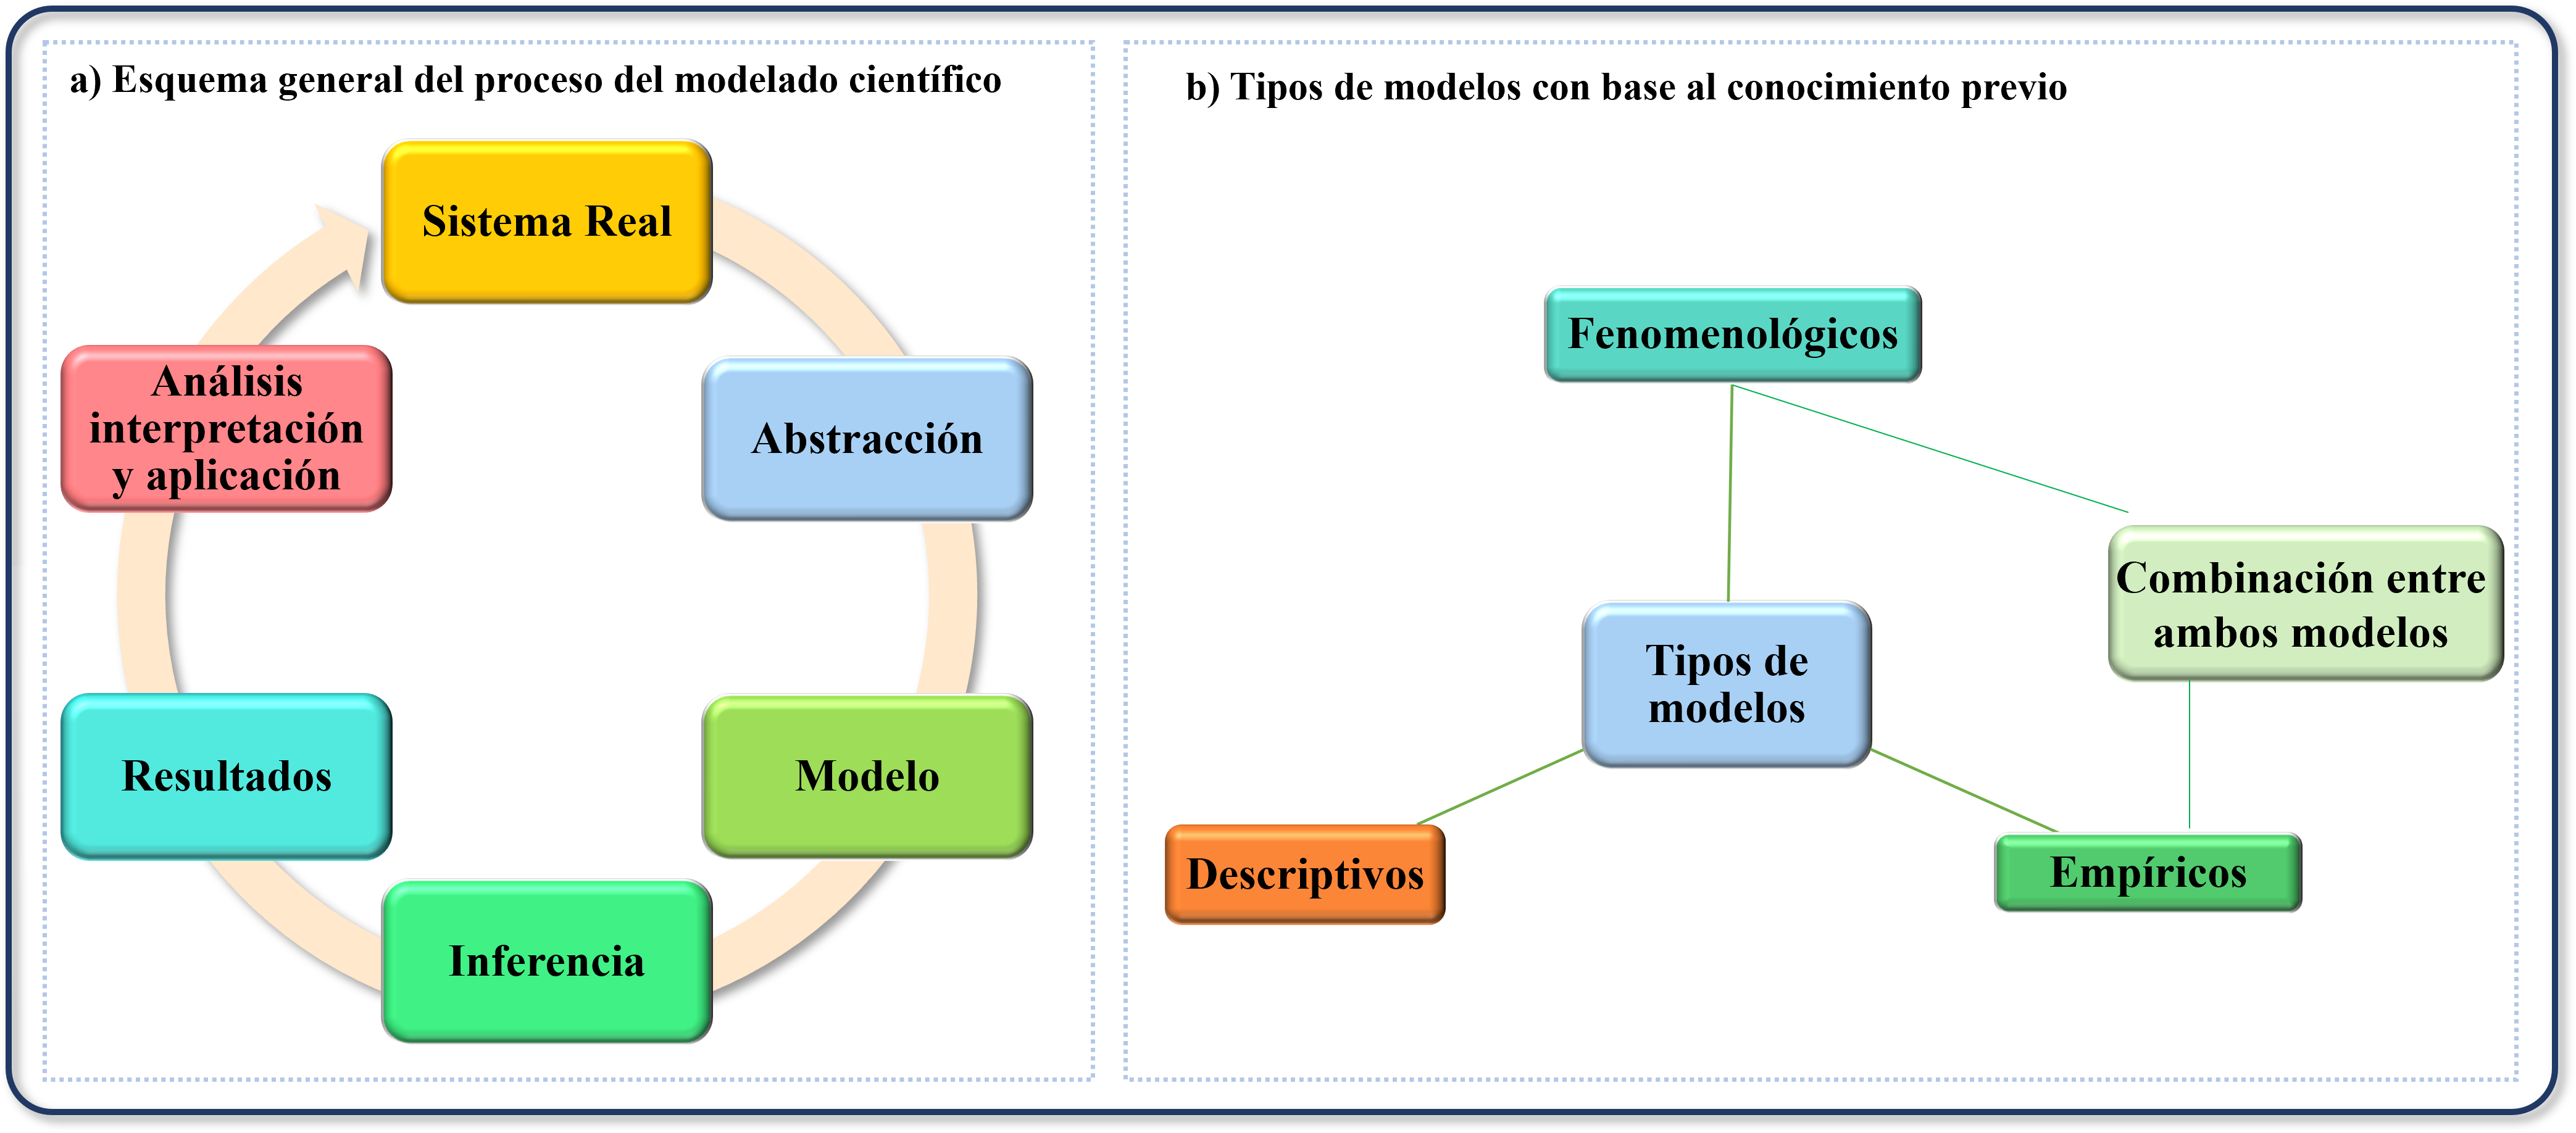
\includegraphics[width=\textwidth, height=8cm]{imagenes/esquema_modelado.png}
    \caption{Sistema de modelado.}
    \label{fig: tipos de modelo}
\end{figure}

Otra forma de modelar un sistema es mediante modelos matemáticos, los cuales replican las relaciones de entrada(s) - salida(s) utilizando expresiones matemáticas. Cuando existe una relación lineal entre la entrada y la salida, el modelo matemático se expresa como:
\begin{equation}
     y(t) = u(t)k_{p}
     \label{eq_modelo}
\end{equation}

Donde $y(t)$ es la salida, $u(t)$ es la entrada del sistema, y $k_{p}$ es la constante de proporcionalidad. No obstante, la ecuación (\ref{eq_modelo}) implica que cualquier cambio en la entrada se reflejará instantáneamente en la salida, lo cual no es cierto en sistemas reales, ya que la salida requiere tiempo para ajustarse. Esta relación se cumple únicamente cuando se ha alcanzado un tiempo suficiente para estabilizarse, conocido como la condición de estado estable, y puede representarse como:\\
\textit{El Valor en estado estable de $u(t)$ = $y(t)$ por el Valor en estado estable de $k_{p}$}
\begin{equation}
    k_{p} = \frac{y(t)}{u(t)}
\end{equation}

Donde $k_{p}$ se refiere a la ganancia del sistema o función de transferencia. Así, una función de transferencia se define como la relación entre la salida en estado estable y la entrada en estado estable de un sistema.

 
\subsection{Formalismo de Euler-Lagrange.}

La formulación Lagrangiana proporciona una forma de modelar la dinámica de un robot al analizar el balance de energía. En este enfoque, el robot se conceptualiza como una entidad cerrada, y las ecuaciones derivadas se centran únicamente en la energía almacenada, representada a través de las energías cinética y potencial. Para un robot dado, los resultados obtenidos mediante esta formulación son idénticos a los obtenidos mediante la formulación de Newton-Euler.
El Lagrangiano es una función escalar definida como la diferencia entre las energías cinética y potencial de un sistema mecánico, en función de las llamadas coordenadas generalizadas \cite{torres2002robots}. En la figura \ref{fig 2_2: Esquema de Euler_lagrange} se desarrolla en detalle la formulación Lagrangiana.


\begin{equation}
J_{i}=
    \begin{bmatrix}
        \lambda_{i} & 1           & 0      &...  & 0  \\
        0           & \lambda_{i} & 1      & ...& 0 \\
        \vdots      & \vdots      & \ddots & \ddots & \vdots \\
             0   &    0    &  ... & \lambda_{i} & 1   \\
           0 &   0   &  ...       &  0   & \lambda_{i} \\
    \end{bmatrix}_{m \times m}
\end{equation}

Donde $J_{i}$ es el bloque de Jordan asociado al eigenvalor $\lambda_{i}$  en $A$ y $m$ es el orden del bloque de Jordan. Esta representación es útil porque simplifica el análisis de la dinámica de sistemas lineales, especialmente cuando $A$ no es diagonalizable. La solución del sistema en términos de la forma de Jordan es:

\begin{equation}
     exp(at) = P exp(Jt) P^{-1} = \sum_{i=1}^{r}\sum_{k=1}^{m_{i}}t^{k-1}exp(\lambda_{i}t)R_{ik}
\end{equation}

Donde $m_{i}$ es el orden del bloque de  Jordan asociado al eigenvalor $A$. El siguiente teorema caracteriza las propiedades de estabilidad del origen.
